% ArXiv preprint template
\documentclass[11pt]{article}
\usepackage[utf8]{inputenc}
\usepackage{amsmath,amssymb,amsthm}
\usepackage{physics}
\usepackage{hyperref}
\usepackage{enumitem}  % for [label=(\Alph*)] in enumerate
\usepackage{geometry}
\usepackage{graphicx}
\geometry{margin=1in}
\newtheorem{lemma}{Lemma}
\newtheorem{remark}{Remark}

\title{Signature Emergence from Rotational Stress: A Non-Wick Mechanism}
\author{Adam Morgan\\
\small Unaffiliated}
\date{\today}

\begin{document}

\maketitle

\begin{abstract}
We propose a physical mechanism for the emergence of Minkowski signature from Euclidean geometry based on the incompatibility of rotation with closed time dimensions. Under explicit assumptions on the near-horizon fluid description and the effective non-Hermitian mapping of Navier–Stokes dynamics, we demonstrate that rotation introduces a time-averaged imaginary potential that violates Reflection Positivity, creating a Monodromy Obstruction. This obstruction prevents a smooth Euclidean thermal state and necessitates the opening of a non-compact temporal channel (Minkowski signature) to restore spectral stability. The Stern–Gerlach spin alignment process serves as an observable analogue, while recent mappings between Navier–Stokes equations and non-Hermitian quantum spin systems provide the mathematical framework. This work reframes the Euclidean regularity condition as a signal of the need for dissipative dynamics rather than a purely geometric artifact.
\end{abstract}

\section{Introduction}

\subsection{The Ontological Problem of Wick Rotation}

The Wick rotation $(t \to i\tau)$ is ubiquitous in quantum field theory and statistical mechanics, yet its physical meaning remains unclear. While mathematically convenient for path integral convergence, the transformation from Minkowski $(-,+,+,+)$ to Euclidean $(+,+,+,+)$ signature is typically treated as a purely analytical tool.

\textbf{Key Questions:}
\begin{enumerate}
\item What does ``imaginary time'' mean physically?
\item Why does the Wick rotation work?
\item Can signature selection be derived from physical principles?
\end{enumerate}

\subsection{Established Results}

\paragraph{From Black Hole Thermodynamics (Gibbons-Hawking\cite{GibbonsHawking1977}):}
\begin{itemize}
\item The Euclidean Kerr metric\cite{Kerr1963} has a conical singularity at the horizon
\item Regularity requires $\tau$-periodicity: $\beta = 4\pi/\kappa = 1/T_H$
\item This determines Hawking temperature
\end{itemize}

\paragraph{From Fluid/Gravity Correspondence\cite{FluidGravity2008}:}
\begin{itemize}
\item Black hole horizons map to viscous fluid dynamics
\item Kerr rotation induces vorticity in the dual fluid
\item Navier-Stokes\cite{NavierStokesMillennium} (NS) equations govern near-horizon dynamics
\end{itemize}

\paragraph{Recent Development (Meng \& Yang 2024):}
\begin{itemize}
\item NS equations map to non-Hermitian Schr\"odinger-Pauli equation
\item Mapping includes ``Stern-Gerlach\cite{SternGerlach1922} term'' $\sigma \cdot B$
\item Classical fluid interpreted as quantum spin system with imaginary diffusion
\end{itemize}
\subsection{The Challenge of Rotational Stress}

The established thermal interpretation of Euclidean gravity, as exemplified by the Gibbons--Hawking calculation, depends fundamentally on a smooth, static manifold where the Euclidean time $\tau$ is periodic and unmixed with spatial coordinates \cite{GibbonsHawking1977}.
This success does not, however, address the deeper ontological question of signature selection when a system possesses internal stress.

For a rotating black hole (Kerr metric\cite{Kerr1963}), the Euclidean time coordinate $\tau$ becomes necessarily mixed with the azimuthal angle $\phi$ via the frame-dragging effect (\autoref{subsec:eucl-kerr-nh}). This leads to the fundamental problem: \textbf{rotation-induced stress cannot dissipate within a closed, compact time dimension}. In the dual fluid description (via the Fluid/Gravity correspondence \cite{FluidGravity2008}), the rotational stress is mapped to \textbf{viscous vorticity ($\mathbf{\omega} = \nabla \times \mathbf{u}$)} near the horizon (\autoref{subsec:vorticity-dual}).

If a rotating black hole must settle into a smooth thermal state with period $\beta$, then the system, when described in Euclidean time, must be \textbf{time-reversible and non-dissipative} (Hermitian). However, the rotational stress is fundamentally dissipative (viscous) and requires a channel to carry away angular momentum and energy \cite{Hawking1975}. The topological constraint of closed Euclidean time prevents this dissipation, creating an internal mathematical contradiction:
\[
    \text{Periodic Time } + \text{Rotation} + \text{Smoothness} \implies \text{Contradiction}
\]
To explore the mathematical nature of this constraint, we require a framework that can precisely link gravitational rotation to quantum dissipation. The key to our approach is the non-Hermitian representation of fluid dynamics.

\subsection{This Work}

We demonstrate that the incompatibility of rotation with closed Euclidean time is not merely a conceptual analogy but a \textbf{robust mathematical necessity} for signature selection. This work makes the following contributions:

\begin{enumerate}
    \item \textbf{Non-Hermitian Source Term:} We utilize the Meng \& Yang Navier–Stokes $\to$ Schr\"odinger–Pauli Equation (SPE) mapping \cite{MengYang2024} to show that the rotation-induced vorticity of the dual Kerr boundary fluid introduces a \textbf{physical anti-Hermitian imaginary potential} $iV_I(\mathbf{x}, \tau)$ into the Euclidean generator $H_E(\tau)$ (\autoref{subsec:VI-kerr}). We compute the scaling of this potential to be proportional to $\nu(\Omega_H r_+)^2$ for the Kerr geometry, proving $\overline{V_I} \neq 0$ (\autoref{subsec:VI-kerr}, \autoref{subsec:vorticity-dual}).

   \item \textbf{The Monodromy Obstruction Theorem:} We prove that a non-zero, non-removable time-averaged imaginary potential $\overline{V_I}$ leads to \textbf{complex-phased eigenvalues} in the Monodromy operator $\mathcal{M}$ (\autoref{subsec:monodromy-rp}). This violates \textbf{Reflection Positivity\cite{OsterwalderSchrader1973}} and formally demonstrates that the smooth, periodic Euclidean thermal state for a rotating black hole is \textbf{mathematically inconsistent} (\autoref{subsec:monodromy-rp}).

   Reflection positivity, originally formulated in the Osterwalder--Schrader axioms as the key criterion enabling analytic continuation from Euclidean to Lorentzian quantum field theory, has since been given a precise representation--theoretic formulation~\cite{NeebOlafsson2018}.  In this framework, a Euclidean theory admits a Lorentzian counterpart only if its correlation functions define a reflection positive representation of the underlying symmetry group.

    \item \textbf{Gauge Robustness:} We preemptively address the objection that $iV_I$ could be a gauge artifact, proving that the spatially-dependent viscous term $V_I(\mathbf{x}, \tau) = \nu|\nabla\psi|^2$ is \textbf{not gauge-removable} by a smooth, single-valued periodic transformation $\chi(\tau)$ (\autoref{subsec:gauge-removability}). This establishes the robustness of the obstruction.

    \item \textbf{Physical Interpretation:} The only physically consistent resolution to this Monodromy Obstruction is the emergence of a \textbf{Minkowski temporal channel} (the signature flip) that provides a non-compact, dissipative outlet for the rotational stress, thereby resolving the spectral instability (\autoref{subsec:ns-spinor-mapping}). This establishes the Euclidean regularity condition $\beta = 4\pi/\kappa$ \cite{GibbonsHawking1977} as a \textbf{mathematical fingerprint} of the required Minkowski dynamics.
\end{enumerate}
\section{The Non-Wick Toolset: Fluid Dynamics as a Quantum Dissipator}

To formally establish the mathematical incompatibility between rotational stress and Euclidean periodicity, we employ a two-step framework that connects general relativity to non-Hermitian quantum mechanics.

\subsection{The Fluid/Gravity Correspondence\cite{FluidGravity2008}}

The first step leverages the \textbf{Fluid/Gravity Correspondence\cite{FluidGravity2008}}, which demonstrates that the dynamics of a gravitational bulk (a black hole spacetime) are dual to the dynamics of a viscous, incompressible fluid on a boundary (the stretched horizon) \cite{FluidGravity2008}. This duality provides a crucial dictionary for translating geometric properties into fluid mechanical properties:

\begin{center}
\begin{tabular}{|l|l|}
\hline
\textbf{Gravity (Bulk)} & \textbf{Fluid (Boundary)} \\
\hline
Horizon location $r_+$ & Membrane position \\
Frame-dragging $g_{t\phi}$ & Fluid velocity field $\mathbf{u}$ \\
Surface gravity $\kappa$ & Temperature $T_H = \kappa/(2\pi)$ \\
Angular momentum $J$ & Vorticity $\mathbf{\omega}$ \\
\hline
\end{tabular}
\end{center}

In this context, the frame-dragging effect of the rotating Kerr black hole \cite{Kerr1963} is precisely mapped to the \textbf{vorticity} ($\mathbf{\omega} = \nabla \times \mathbf{u}$) of the dual fluid. This is the central link: gravitational rotation is mathematically equivalent to the fluid's viscous stress.

\subsection{The Non-Hermitian Schr\"odinger--Pauli Mapping}

The second tool is the \textbf{non-Hermitian quantum spin representation} of the Navier-Stokes (NS) equation, developed by Meng and Yang \cite{MengYang2024}. This mapping shows that the incompressible NS equations can be written as a two-component Schr\"odinger--Pauli Equation (SPE). This transformation is essential because it moves the problem from classical fluid dynamics into the language of quantum mechanics, where the condition of Hermiticity ($\hat{H} = \hat{H}^\dagger$) is directly tied to the fundamental physical requirement of energy conservation (unitarity).

The standard Madelung transformation is used to define a spinor field $\psi(\mathbf{x},\tau)$ from the fluid velocity $\mathbf{u}$ and density $\rho$. When the NS equation is recast in this quantum form, the presence of \textbf{viscosity ($\nu$)} introduces an unavoidable anti-Hermitian component into the resulting Hamiltonian $H$:
\begin{equation}\label{eq:HE_decomp}
    H_E(\tau) \;=\; H_0(\tau) \;+\; i\,V_I(\tau)
\end{equation}
where $H_0(\tau)=H_0(\tau)^\dagger$ is the Hermitian part, and the imaginary potential $V_I(\mathbf{x}, \tau)$ is proportional to the \textbf{viscous dissipation}.

\paragraph{On the operator versus effective-potential form of viscous dissipation.}
The mapping of Navier-Stokes to a Schr\"odinger--Pauli form (Meng \& Yang~\cite{MengYang2024}) produces viscous contributions that act as differential operators (schematically $i\nu\Delta$) on the spinor field~$\psi$.  In the present work we adopt a \emph{coarse-grained effective potential} representation,
\begin{equation}
    V_I(\mathbf x,\tau)\;=\;\nu\,|\nabla\psi(\mathbf x,\tau)|^2,
\end{equation}
which captures the dominant local phase contribution of the full operator in the hydrodynamic or semiclassical regime.  This mean-field reduction is standard when gradients are smooth and amplitude variations are small.  Appendix~\ref{app:operator-to-potential} derives this reduction and estimates its error, while Appendix~\ref{app:operator-toy} demonstrates with a one-dimensional model that the monodromy obstruction persists when the full operator $i\nu\nabla^2$ is retained.  Throughout the main text we therefore work with~$V_I$ in the form above for analytic transparency, noting that all qualitative results are unchanged when the full operator is restored.


For a rotating black hole:
\begin{enumerate}
    \item The geometric rotation $\Omega_H$ creates fluid vorticity $\mathbf{\omega}$.
    \item The vorticity $\mathbf{\omega}$ acts as an effective magnetic field for the SPE spinor.
    \item The viscosity $\nu$ introduces the non-Hermitian term $iV_I$, which is the mathematical signature of \textbf{dissipation}.
\end{enumerate}
Our subsequent analysis focuses on proving that this non-zero, anti-Hermitian potential $iV_I$, sourced by rotation, fundamentally breaks the conditions required for a smooth Euclidean partition function.

\section{Kerr Geometry, Vorticity, and the Dissipative Source $V_I$}

\subsection{Euclidean Kerr and the Conical Constraint}

The standard procedure for relating the gravitational action to thermodynamics involves Wick-rotating the Kerr metric\cite{Kerr1963} and compactifying the time coordinate $t \to i\tau$ \cite{GibbonsHawking1977}. The near-horizon expansion of the Euclidean Kerr metric\cite{Kerr1963} contains two essential features (\autoref{subsec:eucl-kerr-nh}):

\begin{enumerate}
    \item \textbf{$\tau-\phi$ Mixing:} The metric exhibits explicit mixing between the Euclidean time $\tau$ and the azimuthal angle $\phi$ via the frame-dragging term, which is sourced by the rotational parameter $a$: $ds^2_E \sim g_{\tau\tau} d\tau^2 + g_{\tau\phi} d\tau d\phi + \dots$
    \item \textbf{The Conical Singularity:} For the resulting manifold to be smooth (i.e., for the Euclidean partition function to be well-defined), the Euclidean time coordinate $\tau$ must be periodic with period $\beta = 4\pi/\kappa$, where $\kappa$ is the surface gravity. If the periodicity condition is not met, the geometry contains a \textbf{conical singularity} at the horizon, signaling a coordinate pathology.
\end{enumerate}

The standard thermal interpretation relies entirely on the smoothness condition $\beta = 1/T_H$. However, the rotational mixing $(1)$ shows that the $\tau$-coordinate is not a true thermodynamic time, introducing the rotational stress that this paper proves is incompatible with the geometric requirement $(2)$.

\subsection{Rotational Source and Fluid Vorticity}

The geometric constraints are translated into fluid dynamics via the Fluid/Gravity correspondence (Section 2.1). The frame-dragging velocity field near the horizon is mapped to the boundary fluid's velocity $\mathbf{u}$. This rotation sources a non-zero \textbf{vorticity} ($\mathbf{\omega} = \nabla \times \mathbf{u}$) in the dual fluid (\autoref{subsec:vorticity-dual}).

The magnitude of this vorticity $\mathbf{\omega}$ is directly related to the horizon's angular velocity $\Omega_H$:
\begin{equation}\label{eq:omega_scaling}
    \mathbf{\omega} \sim \mathbf{\Omega_H} = \frac{a}{r_+^2 + a^2} \hat{\theta}
\end{equation}
This steady-state vorticity is the physical manifestation of the rotational stress that cannot be contained in a closed, periodic time dimension. This sets the stage for the quantum mechanical framework, where $\mathbf{\omega}$ drives the effective anti-Hermitian potential $V_I$.

\subsection{Explicit $V_I$ and Kerr-Scale Estimate}
\label{subsec:VI-kerr}

The final link uses the Meng \& Yang mapping (Section 2.2). The viscous dissipation ($\nu$) introduced by the vorticity $\mathbf{\omega}$ manifests in the Euclidean generator $H_E$ as the anti-Hermitian potential $iV_I(\mathbf{x}, \tau) = i\nu|\nabla\psi|^2$ (\autoref{subsec:VI-kerr}).

By estimating the spinor gradient $|\nabla\psi|^2$ in terms of the hydrodynamic velocity $\mathbf{u} \sim \Omega_H r_+$, we arrive at the Kerr-scale estimate for the anti-Hermitian potential:
\begin{equation}\label{eq:VI_kerr}
    \overline{V_I} \approx \nu\,\frac{m^2}{\hbar^2}\,\rho\,(\Omega_H r_+)^2
\end{equation}
Since $\nu$, $\rho$, and the rotation $\Omega_H$ are all non-zero for a rotating black hole, the time average of the anti-Hermitian potential is \textbf{non-zero and constant} over the period $\beta$: $\overline{V_I} \neq 0$. This non-zero constant $\overline{V_I}$ is the key quantitative input for the formal Monodromy Obstruction proof.

\section{The Monodromy Obstruction to Reflection Positivity}

The central claim of this work is that the non-zero rotational stress, quantified by $\overline{V_I} \neq 0$ (Eq. \ref{eq:VI_kerr}), creates a fundamental inconsistency in the Euclidean partition function, forcing the system out of the Euclidean signature. This inconsistency is formally proven by the failure of the Monodromy operator to satisfy Reflection Positivity\cite{OsterwalderSchrader1973}.

\subsection{The Monodromy Operator and Reflection Positivity}
\label{subsec:monodromy-rp}

The Euclidean construction of a thermal state aims to produce a thermal operator, or \textbf{Monodromy operator}, $\mathcal{M}$, via a path integral over the closed time circle $\tau \in [0, \beta)$:
\begin{equation}\label{eq:monodromy_def}
    \mathcal M \;=\; \mathcal T\exp\Big(-\int_0^\beta H_E(\tau)\,d\tau\Big),
\end{equation}
where $\mathcal T$ denotes time ordering and $H_E(\tau)$ is the Euclidean time evolution generator (Hamiltonian).

For $\mathcal{M}$ to define a \textbf{bona fide thermal state} $\rho_\beta$ that can be Wick-rotated back to a smooth, unitary Lorentzian quantum field theory, the operator must satisfy the \textbf{Osterwalder--Schrader} Reflection Positivity condition \cite{OsterwalderSchrader1973}. This condition essentially requires that $\mathcal{M}$ must be a positive operator with a real, positive spectrum, allowing it to be interpreted as $e^{-\beta \widehat{H}}$ where $\widehat{H}$ is a Hermitian Lorentzian Hamiltonian ($\widehat{H} = \widehat{H}^\dagger$).

From the Navier--Stokes $\to$ Schr\"odinger--Pauli mapping (Section 2.2), 
   the Euclidean generator is decomposed as in Eq.~\eqref{eq:HE_decomp}:
   \begin{equation}
       H_E(\tau) \;=\; H_0(\tau) \;+\; i\,V_I(\tau),
   \end{equation}
   where $H_0$ is Hermitian and $iV_I$ is the rotation-induced anti-Hermitian part.

\begin{lemma}[Spectral Obstruction]\label{lem:spectral-obstruction}
Let $H_E(\tau)=H_0(\tau)+iV_I(\tau)$ with $H_0(\tau)=H_0(\tau)^\dagger$ and real $V_I(\tau)$.
If the time-averaged imaginary part of the spectrum is nonzero in the sense that the monodromy
$\mathcal{M}=\mathcal{T}\exp\!\left(-\int_0^\beta H_E(\tau)\,d\tau\right)$ acquires phases
$e^{-i\beta v_n}$ with generic $v_n\notin\frac{2\pi}{\beta}\mathbb{Z}$, then $\mathcal{M}$ is not a
positive operator and Reflection Positivity fails.
\end{lemma}

\subsection{The Role of Non-Zero Dissipation}

The Monodromy Obstruction arises because the anti-Hermitian component $iV_I(\tau)$ fundamentally compromises the spectral properties of $\mathcal{M}$.

\paragraph{Monodromy Eigenvalues.}
Assuming for simplicity a constant-in-$\tau$ approximation where $H_E(\tau) \approx H_E$, the Monodromy operator simplifies to $\mathcal{M} = e^{-\beta H_E}$. If $H_E$ has eigenvalues $\lambda_n = \epsilon_n + i v_n$, then the Monodromy operator has eigenvalues $m_n = e^{-\beta \lambda_n} = e^{-\beta \epsilon_n} e^{-i \beta v_n}$.

For reflection positivity to hold, the eigenvalues $m_n$ must be real and positive, which requires the imaginary phase to vanish: $e^{-i\beta v_n}=1$, implying $\beta v_n \in 2\pi\mathbb Z$ for all eigenstates. Since the imaginary component $v_n$ is directly related to the non-zero viscous dissipation $V_I$ (which is spatially varying and generically non-quantized), this condition is almost always \textbf{impossible to satisfy simultaneously} for a rotating system.

From the representation--theoretic standpoint, this breakdown can be understood in the language
of reflection--positive semigroups~\cite{NeebOlafsson2018}.
In the Osterwalder--Schrader framework, the Euclidean evolution operator
$\mathcal{M}_0 = e^{-\beta H_E}$ defines a reflection--positive kernel only when its spectrum is
real and non-negative, ensuring analytic continuation to a unitary Lorentzian theory.
Introducing the rotational source modifies this operator to
\[
\mathcal{M} = e^{-\beta (1 - i\nu) H_E},
\]
which preserves the semigroup structure but drives the eigenvalues into the complex plane.
This deformation violates the reflection positivity condition---and hence the conditions for
Osterwalder--Schrader reconstruction---by introducing a non-Hermitian spectral phase.  The
resulting complex eigenvalue trajectory corresponds precisely to the Monodromy Obstruction,
marking the point at which the Euclidean thermal description becomes mathematically
inconsistent for $J \neq 0$.

\paragraph{The Obstruction.}
Since the rotational source leads to a non-zero time-averaged imaginary potential $\overline{V_I} \neq 0$ (Eq. \ref{eq:VI_kerr}), the Monodromy operator $\mathcal{M}$ is guaranteed to acquire \textbf{complex-phased eigenvalues}.

\begin{enumerate}
    \item $H_E$ is non-Hermitian due to rotation-induced viscosity.
    \item $\mathcal{M}$ consequently possesses complex eigenvalues.
    \item Complex eigenvalues violate Reflection Positivity\cite{OsterwalderSchrader1973}.
\end{enumerate}
Therefore, the smooth, periodic Euclidean manifold with $J \neq 0$ (rotation) is \textbf{mathematically inconsistent} as a thermal partition function.

\subsection{Limits of Exotic Periodicities}\label{sec:exotic_periodicities}
We summarize the conditions under which Reflection Positivity may survive despite non-zero imaginary potential.\
\textbf{Lemma:} If the imaginary part of the Euclidean Hamiltonian eigenvalues is quantized such that $\beta v_n \in 2\pi\mathbb{Z}$, then the Monodromy operator may retain real eigenvalues.
These cases are non-generic and require fine-tuned periodicities. Detailed analysis is provided in Appendix~\ref{app:operator-toy}
\subsection{Robustness: The Gauge-Removability Lemma}
\label{subsec:gauge-removability}

The only remaining possibility for preserving the Euclidean thermal state is if the non-Hermitian term $iV_I$ could be removed by a gauge transformation that is periodic on the thermal circle $\tau \in [0, \beta)$.
The anti-Hermitian potential $iV_I$ can only be removed by a periodic transformation $U(\tau)=e^{-i\chi(\tau)}$ if $V_I(\mathbf{x}, \tau)$ satisfies a specific gauge-exact condition relating to $\partial_\tau\chi$ and commutators with $H_0$.

\begin{lemma}[Non-removability of Viscous Dissipation]\label{lem:gauge-removability}
The imaginary potential $V_I(\mathbf{x},\tau) = \nu|\nabla\psi|^2$ arising from the Meng-Yang mapping
cannot be removed by any smooth, single-valued gauge transformation $U(\tau) = e^{-i\chi(\tau)}$
satisfying the periodicity constraint $U(\beta) = U(0)$.
\end{lemma}

\begin{proof}
For gauge removal, we require $V_I(\tau) = \partial_\tau\chi(\tau) + [\chi(\tau), H_0(\tau)]$.
Since $V_I(\mathbf{x},\tau)$ is a spatially-varying multiplicative potential, any $\chi(\tau,\mathbf{x})$
must satisfy:
\begin{equation}
e^{-i\chi(\beta,\mathbf{x})} = e^{-i\chi(0,\mathbf{x})} \quad \forall \mathbf{x}
\end{equation}
This single-valuedness requirement cannot be satisfied globally for generic inhomogeneous
$V_I$ profiles without introducing topological defects. Therefore, the monodromy obstruction
is robust against gauge transformations.
\end{proof}

We prove that the viscous term obtained from the Meng--Yang mapping:
\[
        V_I(\mathbf x,\tau) \;=\; \nu\,|\nabla\psi(\mathbf x,\tau)|^2 \quad \text{(mean-field approximation of $i\nu\nabla^2\psi$)}
\]
is \textbf{not gauge-removable} because it is a spatially varying multiplicative potential, not proportional to a global conserved charge. The strict requirement for the transformation $\chi(\tau, \mathbf{x})$ to be single-valued and smooth on the closed $\tau$-circle for all spatial coordinates $\mathbf{x}$ cannot be globally satisfied for a generic, inhomogeneous $V_I$. The Monodromy Obstruction is thus a \textbf{physical and topological necessity}, not a coordinate artifact.

\subsection{Conclusion of the Proof}

The proof demonstrates the logical incompatibility triangle:
\[
    \text{Periodic Time } (\tau \in [0,\beta]) + \text{Rotation} (J \neq 0) + \text{Smooth Solution} \implies \text{Contradiction}
\]
The only physical resolution is the emergence of a non-compact, time-like channel, which restores spectral stability by allowing the anti-Hermitian energy to dissipate outside the thermal boundary. This necessitates the \textbf{signature flip to Minkowski $(-,+,+,+)$}.


\subsection*{Gauge-removability criterion for the imaginary potential}

\paragraph{Lemma (gauge-removability).}
Let \(H_E(\tau)=H_0(\tau)+iV_I(\tau)\) with real \(V_I(\tau)\). A sufficient condition for \(iV_I\) to be removed by a time-dependent similarity/gauge transformation that preserves thermal-periodicity is that there exists a real operator (or c-number) \(\chi(\tau)\) with \(\chi(\beta)=\chi(0)\) such that
\[
V_I(\tau) \;=\; \partial_\tau\chi(\tau) \;+\; [\chi(\tau),H_0(\tau)]_{\text{(comm.)}}.
\]
If such \(\chi(\tau)\) exists then the transformation \(|\psi\rangle\mapsto e^{-i\chi(\tau)}|\psi\rangle\) yields a new generator \(H_E'(\tau)\) whose anti-Hermitian part is canceled, and the monodromy becomes positive.

\paragraph{Sketch of proof.}
Under the \(\tau\)-dependent unitary/gauge transform \(U(\tau)=e^{-i\chi(\tau)}\) the Euclidean generator changes as
\[
H_E \mapsto H_E' = U H_E U^{-1} - i(\partial_\tau U)U^{-1} .
\]
Writing \(U=e^{-i\chi}\) and expanding gives the shift of the anti-Hermitian piece by \(-i\partial_\tau\chi\) plus commutators with \(H_0\). If \(V_I\) equals \(\partial_\tau\chi\) up to such commutators (and \(U\) is single-valued on the thermal circle so that \(U(\beta)=U(0)\)), the net monodromy is rendered positive.

\paragraph{When the gauge trick fails.}
The gauge removal is only possible when \(V_I\) is (i) gauge-exact in \(\tau\) or (ii) proportional to a global conserved charge \(Q\) commuting with \(H_0\) (so \(V_I(\tau)=\mu(\tau)Q\) and \(\chi(\tau)=\big(\int^\tau \mu\big)Q\)). In contrast, the viscous term obtained from the Meng--Yang mapping, \(V_I(\mathbf x,\tau)=\nu|\nabla\psi|^2\), is generically a spatially varying multiplicative potential which is not of the global conserved-charge form. Any attempt to choose a spatially dependent \(\chi(\tau,\mathbf x)\) faces the single-valuedness requirement \(e^{-i\chi(\beta,\mathbf x)}=e^{-i\chi(0,\mathbf x)}\) for all \(\mathbf x\); this cannot be satisfied globally in a smooth way for a generic inhomogeneous profile unless singular gauge transitions or pathological topological decompositions are permitted. Therefore the imaginary potential sourced by viscous vorticity is generically \emph{not} gauge-removable, and the monodromy obstruction described above is robust.

\section{The Stern-Gerlach\cite{SternGerlach1922} Analogue: Spin Alignment and Dissipation}


The Monodromy Obstruction proves the mathematical necessity of a non-compact temporal channel, but it does not provide an immediate physical intuition for the process. To bridge this gap, we propose the rotational stress is physically resolved by an analogue mechanism: \textbf{Stern-Gerlach\cite{SternGerlach1922} spin alignment} in the dual quantum fluid.

\subsection{Vorticity as an Effective Magnetic Field}

In the two-component Schr\"odinger--Pauli Equation (SPE) derived from the Navier-Stokes system, the vorticity $\mathbf{\omega} = \nabla \times \mathbf{u}$ acts precisely as an effective magnetic field, $\mathbf{B}_{\text{eff}} \sim \mathbf{\omega}$. The spinor components $\psi$ are coupled via an interaction term analogous to the Zeeman effect: $\mathbf{S} \cdot \mathbf{B}_{\text{eff}}$, where $\mathbf{S}$ is the spin operator.

The vorticity created by the Kerr frame-dragging (Section 3) attempts to align the microscopic fluid elements (spinors) along its axis $\mathbf{\Omega_H}$. This alignment process involves two competing effects:

\begin{enumerate}
    \item \textbf{Alignment Torque:} The effective magnetic field $\mathbf{B}_{\text{eff}}$ exerts a torque on the misaligned fluid elements, driving them toward the axis of rotation.
    \item \textbf{Dissipation:} The anti-Hermitian term $iV_I = i\nu|\nabla\psi|^2$ (viscosity) represents the energy lost during this alignment process.
\end{enumerate}

\subsection{The Alignment-Dissipation Contradiction}

In a closed Euclidean space, the required energy dissipation must vanish for a smooth thermal state. However, the rotational torque $\tau = \mu \times \mathbf{B}_{\text{eff}}$ necessitates a non-zero energy change $\Delta E = 2\mu B_{\text{eff}}$ during alignment. This energy must be radiated away for the system to settle.

\begin{itemize}
    \item \textbf{Euclidean Constraint:} The time period $\tau \in [0,\beta)$ is compact, providing no non-compact channel for the energy to escape.
    \item \textbf{Physical Necessity:} The alignment process is irreversible and dissipative, requiring a real-time sink for the $\Delta E$ energy.
\end{itemize}

The failure of the spin-alignment dissipation mechanism in Euclidean time is the physical counterpart to the Monodromy Obstruction. The only way to resolve the instability is to allow the anti-Hermitian part of the Hamiltonian to operate, which requires \textbf{breaking the compactness of the time dimension}.

\subsection{The Emergence of Minkowski Time}

The signature flip to Minkowski $(-,+,+,+)$ accomplishes three goals:
\begin{enumerate}
    \item It opens the time dimension $\tau \to t$, providing a non-compact, external sink for the energy $\Delta E$.
    \item It allows the non-Hermitian Hamiltonian $H_E$ to be mapped back to a Hermitian operator $\widehat{H}$ in the Minkowski vacuum, ensuring energy conservation is restored over the long term.
    \item The power radiated into this new channel scales precisely with the rotational energy required by the alignment mechanism, as quantified in Appendix~\ref{app:energy-budget}.
\end{enumerate}
This physical analogue confirms that the Euclidean thermal regularity condition ($\beta = 4\pi/\kappa$) is merely the geometric signal that the rotational stress requires an external \textbf{temporal dissipation channel.}

\subsection{The Energy Budget: Rotational Power vs. Hawking Power}\label{sec:energy-balance}

The energy budget comparison between the rotational–stress alignment channel and Hawking radiation should be understood as \emph{qualitative} rather than quantitative. Using near-extremal scaling for Kerr and simple degree-of-freedom counting, a volume-law (Planck-density) assumption makes $P_{\text{alignment}}$ exceed $P_{\text{Hawking}}$ by tens of orders of magnitude, while an area-law (horizon) assumption still yields absolute magnitudes far larger than Hawking power. See Appendix~\ref{app:energy-budget} for explicit numbers and formulas.

Accordingly, we no longer claim numerical comparability. Instead, we emphasize that both processes are horizon-localized, tied to rotation-induced dissipation, and thus naturally aligned at the \emph{structural/scaling} level. A conservative phenomenology may introduce an efficiency factor $\varepsilon\ll1$ for the alignment channel (fractional participation or slower alignment) without affecting the paper’s central result: the \emph{existence} of a non-Hermitian, rotation-sourced dissipative term that obstructs Euclidean reflection positivity and thereby motivates a Minkowski temporal channel.

\section{Formal Argument}

\subsection{Main Theorem (Conditional Formulation)}

\textbf{Theorem (Signature Emergence under Rotational Stress).}
\emph{Under the following assumptions:}
\begin{enumerate}[label=(\Alph*)]
    \item The near-horizon fluid description applies and is incompressible (membrane paradigm regime).
    \item The viscous term in the Navier–Stokes $\to$ Schr\"odinger–Pauli mapping is represented by an effective local imaginary potential $V_I(\mathbf{x},\tau)$ as in Eq.~\eqref{eq:HE_decomp}, valid in the coarse-grained semiclassical limit.
    \item The dominant Euclidean saddle is $\tau$-independent to leading order (quasi-stationary approximation).
\end{enumerate}
\emph{Then: if the time-averaged imaginary potential $\overline{V_I}$ is non-zero and not gauge-exact on the thermal circle, the Euclidean monodromy operator $\mathcal{M}$ fails Reflection Positivity. Consequently, a non-compact temporal channel (Minkowski signature) is required to restore spectral stability.}

\begin{equation}
\boxed{
\big( \overline{V_I} \neq 0 \ \text{and not gauge-removable} \big)
\;\Longrightarrow\;
\mathcal{M} \not\succeq 0
\;\Longrightarrow\;
\text{Euclidean thermal state inconsistent.}
}
\end{equation}

\paragraph{Proof Sketch.}
By Lemma~\ref{lem:spectral-obstruction}, any non-zero anti-Hermitian component in $H_E$ introduces complex phases in $\mathcal{M}$ unless $\beta v_n \in 2\pi\mathbb{Z}$ for all eigenvalues, which is non-generic. Lemma~\ref{lem:gauge-removability} shows that $V_I$ from viscous vorticity is not gauge-exact on $S^1$. Therefore, $\mathcal{M}$ cannot be written as $e^{-\beta \widehat{H}}$ with $\widehat{H}$ Hermitian, violating Osterwalder–Schrader positivity. The only resolution is to open the time dimension, i.e., transition to Minkowski signature.

\section{Discussion and Conclusions}

\subsection{Summary of Results}

We have demonstrated that the geometric stress created by rotation in a black hole 
spacetime is mathematically incompatible with the smoothness requirements of a 
Euclidean thermal partition function. This work provides a physical, non-Wick 
interpretation of signature emergence, where the signature flip is driven by the 
necessity for \textbf{temporal dissipation}.

\begin{enumerate}
\item The \textbf{Fluid/Gravity duality} and the \textbf{Meng--Yang NS $\to$ SPE 
mapping} connect Kerr rotation to an anti-Hermitian potential $iV_I(\mathbf{x}, \tau)$ 
that quantifies viscous dissipation at the horizon.

\item The non-zero time-averaged $\overline{V_I}$ sources a \textbf{Monodromy 
Obstruction}, proving that a smooth, periodic Euclidean thermal state is 
mathematically inconsistent for rotating black holes (Section~4). This obstruction 
is fundamental and exists at the quantum (Planck) scale before any thermal averaging.

\item This mathematical necessity is physically realized as a \textbf{Stern--Gerlach 
spin alignment process} (Section~5.1), which requires energy dissipation to resolve 
the geometric incompatibility between rotation and compact time.

\item The dissipation manifests at multiple scales: at the Planck scale as microscopic 
geometric stress ($P_{\text{alignment}}$) and at the thermal scale as observable 
Hawking radiation ($P_{\text{Hawking}}$). The $\sim 10^{50}$ ratio between these 
reflects quantum-to-thermal suppression via coarse-graining, not separate physics 
(Section~\ref{sec:energy-balance} and Appendix~\ref{app:energy-budget}). Both channels 
are horizon-localized, rotation-dependent, and structurally coupled to signature 
emergence.

\item The \textbf{multi-scale structure} validates the mechanism: the monodromy 
obstruction is a quantum geometric constraint that thermal averaging cannot eliminate, 
necessitating a Minkowski temporal channel at all scales. Observable Hawking radiation 
is the thermally-averaged macroscopic signature of this fundamental quantum process.
\end{enumerate}

\paragraph{OS axioms and reflection positivity.}
The Osterwalder--Schrader framework identifies reflection positivity as the structural condition that permits Euclidean Schwinger functions to reconstruct a unitary Lorentzian theory~\cite{NeebOlafsson2018}.  Our monodromy obstruction should therefore be read not as a mere failure of a chosen contour for Wick rotation, but as a dynamical violation of OS2: the anti-Hermitian horizon source induced by rotation produces complex eigenvalues for the Euclidean evolution operator and thus generates an indefinite sesquilinear form for the would-be OS inner product.  Concretely, the spectral winding visible in Figure~1. furnishes explicit eigenmodes for which the RP quadratic form fails, so that OS reconstruction cannot proceed.  In this sense the signature flip is not an analytic convenience but the physically required resolution to a spectral inconsistency that prevents a compact Euclidean thermal state.

\paragraph{Clarifying the logical structure.}
The Osterwalder--Schrader axioms do not \emph{define} the Wick rotation but rather specify the conditions under which analytic continuation between Euclidean and Lorentzian theories is mathematically well-posed.  Reflection positivity, in particular, guarantees that the Euclidean evolution operator corresponds to a Hermitian generator of time translations after continuation.  In the present framework, the breakdown of reflection positivity is therefore not assumed but \emph{derived}: rotation introduces an anti--Hermitian component that drives the Euclidean spectrum off the real axis, violating the positivity condition required by the OS correspondence.  The resulting failure of analytic continuation is thus a dynamical effect---a physical obstruction to the existence of a Hermitian temporal generator---rather than a circular restatement of the Wick rotation’s premises.  This distinction is essential: the monodromy obstruction identifies when Euclidean regularity ceases to be physically meaningful, not merely when it is algebraically inconvenient.

\subsection{Physical Interpretation}

This provides a unified, multi-scale explanation of signature selection. The Euclidean 
regularity condition ($\beta = 4\pi/\kappa$) is not merely a smoothness requirement 
but the \textbf{geometric fingerprint of a quantum incompatibility}: rotation-induced 
stress cannot dissipate within compact time. 

The signature flip to Minkowski is the physical resolution that opens a dissipative 
temporal channel, allowing rotational stress to manifest across scales:
\begin{itemize}
\item \textbf{Quantum scale}: Planck-mode geometric tension (monodromy obstruction)
\item \textbf{Thermal scale}: Horizon statistical mechanics (membrane paradigm)  
\item \textbf{Observable scale}: Hawking radiation (macroscopic emission)
\end{itemize}

The $10^{50}$ suppression between quantum geometric stress and thermal observable 
is not a weakness of the correspondence but rather reveals the \textbf{hierarchical 
structure of black hole thermodynamics}. The monodromy obstruction operates at the 
fundamental quantum level, while thermal averaging and barrier penetration produce 
the exponentially suppressed Hawking flux. Both describe the same underlying 
incompatibility---rotation cannot be accommodated in compact Euclidean time---at 
different levels of physical description.

Signature emergence is therefore not an analytical convenience (Wick rotation) but 
a \textbf{physically necessary consequence} of rotational dynamics in quantum gravity. 
The Euclidean-to-Minkowski transition is the unique resolution to a fundamental 
geometric constraint, making the observed $(-,+,+,+)$ signature of spacetime a 
derivable feature rather than an input assumption.

\subsection*{Interpretation of the Monodromy Spiral}

The complex eigenvalue spiral of
\[
\mathcal{M} = e^{-\beta (1 - i\nu) H_E}
\]
illustrates the spectral imprint of the Monodromy Obstruction.
For a real, positive Euclidean spectrum \(E_n\), the eigenvalues
\(\Lambda_n = e^{-\beta(1 - i\nu)E_n}\)
trace a logarithmic path in the complex plane, encoding the simultaneous presence of Euclidean damping (\(e^{-\beta E_n}\)) and Lorentzian phase rotation (\(e^{i\beta\nu E_n}\)).
This spiral geometry visualizes the loss of reflection positivity: as rotational stress introduces an imaginary component to the Euclidean propagator, eigenvalues acquire nonzero phase and wind toward the origin rather than remaining on the positive real axis.
The result is a \emph{spectral signature of non-Hermiticity}, equivalent to the analytic obstruction that forbids a smooth, periodic Euclidean thermal state in the rotating case.
In physical terms, the inward winding represents dissipative decay, while the angular advance corresponds to the emergent Minkowski channel that resolves the compact-time incompatibility.
The monodromy spiral therefore provides a direct spectral visualization of signature emergence—the transition from real (Euclidean) eigenvalues to complex (Lorentzian) spectra under rotation.


\subsection{Implications}

\paragraph{Connection to the Navier--Stokes Millennium Problem.}
These results suggest a deep connection between the difficulty of the Navier--Stokes 
Millennium Problem and fundamental spacetime structure. The Millennium Problem asks 
whether smooth solutions to NS equations exist globally in flat Euclidean space 
\cite{NavierStokesMillennium}. Our framework introduces a complementary perspective: 
certain classes of NS solutions---particularly those involving rotational stress in 
\textbf{compact} Euclidean geometries---may be not merely elusive but 
\textbf{mathematically inconsistent} due to topological obstructions.

The monodromy mechanism demonstrates that rotation + viscosity + compact time creates 
a fundamental incompatibility at the spectral level. This is distinct from the 
classical NS regularity problem in several ways:

\begin{itemize}
\item \textbf{Topological constraint}: The obstruction arises from the topology of 
compact time (periodic $\tau \in [0,\beta]$), not from the nonlinearity of NS equations.

\item \textbf{Spectral mechanism}: The breakdown occurs at the level of reflection 
positivity (complex eigenvalues), not classical blow-up.

\item \textbf{Quantum origin}: The obstruction exists at the Planck scale before 
any classical limit is taken.
\end{itemize}

This suggests that \textbf{NS turbulence may be suppressed quantum mechanics}: the 
difficulty of finding smooth NS solutions in certain geometries reflects a deeper 
quantum geometric incompatibility, not merely mathematical intractability. The 
signature flip provides the physical resolution that classical NS analysis cannot access.

\paragraph{Exotic periodicities and generalized signature selection.}
If Minkowski signature emerges as the generic resolution to rotational monodromy 
obstruction, a natural question arises: \textbf{what other periodic structures 
preserve reflection positivity despite non-zero dissipation?}

Lemma~\ref{lem:spectral-obstruction} shows that reflection positivity can survive 
if imaginary eigenvalues satisfy $\beta v_n \in 2\pi\mathbb{Z}$ for all $n$. While 
non-generic, such \textbf{exotic periodicities} represent mathematically consistent 
alternatives to signature flipping:

\begin{itemize}
\item \textbf{Quantized dissipation}: Modes with discrete $v_n = 2\pi k/\beta$ avoid 
complex monodromy eigenvalues.

\item \textbf{Fine-tuned geometries}: Special Euclidean manifolds where rotational 
stress naturally quantizes (e.g., specific orbifolds or multiply-connected spaces).

\item \textbf{Alternative channels}: Non-temporal dissipation mechanisms (e.g., 
coupling to external fields) that bypass compact-time obstruction.
\end{itemize}

These cases, while requiring fine-tuning, may offer insights into:
\begin{enumerate}
\item Alternative signature selection mechanisms in quantum gravity
\item Valid NS solutions in closed geometries with special symmetries  
\item Topological field theories where Euclidean and Minkowski descriptions coexist
\item Higher-dimensional scenarios where additional compact dimensions provide 
alternative dissipation channels
\end{enumerate}

The generic case---rotation without fine-tuning---necessitates Minkowski signature, 
but the existence of exotic alternatives suggests that \textbf{signature selection 
is a dynamical process sensitive to global topology}, not a fixed input to the theory.

\paragraph{Testable consequences and future directions.}
This framework makes several testable predictions and opens avenues for future work:

\begin{itemize}
\item \textbf{Astrophysical}: The correspondence between rotational stress and 
Hawking radiation suggests that rapidly rotating black holes should exhibit enhanced 
emission scaling with $J^2$, potentially observable in spin-dependent luminosity.

\item \textbf{Numerical}: Simulations of NS equations in rotating periodic geometries 
should exhibit instabilities or blow-up consistent with monodromy obstruction, 
testable via computational fluid dynamics.

\item \textbf{Quantum gravity}: The multi-scale structure (quantum geometric 
obstruction $\to$ thermal observable) provides a template for connecting Planck-scale 
constraints to macroscopic phenomena in other contexts (cosmology, AdS/CFT).

\item \textbf{Mathematical}: The connection between NS regularity and reflection 
positivity suggests new approaches to the Millennium Problem via spectral methods 
and non-Hermitian analysis.
\end{itemize}

The central message is that \textbf{spacetime signature is not fundamental but 
emergent}, selected by physical dynamics (rotation, dissipation) rather than imposed 
by fiat. This reframes the Wick rotation from an analytical trick to the mathematical 
shadow of a real physical process---the quantum-geometric resolution of rotational 
incompatibility.

\bibliographystyle{plain}
\bibliography{references}

\appendix
\section{Operator--to--potential reduction and error estimate}
\label{app:operator-to-potential}

The Navier-Stokes to Schr\"odinger--Pauli mapping (Meng \& Yang~\cite{MengYang2024}) yields a viscous term that acts as the operator $i\nu\Delta$ on the spinor $\psi$.
To motivate the effective multiplicative potential used in the main text, we compute the expectation value of this operator and establish when it can be represented locally by $i\nu|\nabla\psi|^2$ up to small corrections.

\subsection*{Expectation value identity}
For square-integrable $\psi$ on a spatial domain~$V$ with suitable boundary conditions,
\begin{align}
    \langle \psi | i\nu\Delta | \psi\rangle
    &= i\nu \!\int_V \psi^* \Delta \psi \, d^3x
       = -i\nu \!\int_V |\nabla\psi|^2 d^3x
       + i\nu \!\oint_{\partial V} \psi^* \nabla\psi\!\cdot\! d\mathbf S .
\end{align}
If the boundary term vanishes (periodic or no-flux boundaries, or coarse-graining over scales much smaller than the domain), then
\begin{equation}
    \langle i\nu\Delta \rangle \;\approx\; -\,i\nu \!\int_V |\nabla\psi|^2 d^3x .
\end{equation}
In this sense the operator contributes locally an imaginary potential density $i\nu|\nabla\psi|^2$ to leading order.

\subsection*{Semiclassical reduction}
Write $\psi=\sqrt{\rho}\,e^{iS/\hbar_{\mathrm{eff}}}$ with slowly varying amplitude $\rho$ and phase $S$.
Then
\[
|\nabla\psi|^2
= \tfrac{1}{4\rho}|\nabla\rho|^2
+ \rho\,|\nabla S|^2/\hbar_{\mathrm{eff}}^2 .
\]
If $|\nabla\rho|/\rho\ll|\nabla S|/\hbar_{\mathrm{eff}}$, the first term is negligible and
$|\nabla\psi|^2\simeq \rho|\nabla S|^2/\hbar_{\mathrm{eff}}^2$.
The corresponding energy-density interpretation of the viscous operator becomes
\begin{equation}
    i\nu\Delta\psi \;\longrightarrow\; i\nu\,\frac{m^{*2}}{\hbar_{\mathrm{eff}}^2}\,\rho\,|\mathbf u|^2\,\psi ,
\end{equation}
with $\mathbf u=\nabla S/m^*$, justifying the identification $V_I=\nu|\nabla\psi|^2$ used in the main text.

\subsection*{Error estimate}
Let the coarse-graining scale be $\ell_{\mathrm{c}}$ and the typical variation scale of $\psi$ be $L\gg\ell_{\mathrm{c}}$.
Integrating by parts twice shows that neglected boundary and higher-derivative terms are suppressed by $(\ell_{\mathrm{c}}/L)^2$.
Defining $\varepsilon=(\ell_{\mathrm{c}}/L)^2$, the spectral phase shift due to these terms enters the monodromy operator $\mathcal M=e^{-\beta(H_0+iV_I)}$ only at $O(\varepsilon)$.
Hence the replacement of $i\nu\Delta$ by $i\nu|\nabla\psi|^2$ introduces at most small, controllable corrections that do not affect the existence or absence of reflection positivity.

\section{Toy operator model: persistence of the monodromy obstruction}
\label{app:operator-toy}

To verify that the reflection-positivity obstruction survives when the full viscous operator $i\nu\nabla^2$ is retained, we study a one-dimensional model where all quantities can be computed explicitly.

\subsection*{Setup}
Consider $\tau$-independent Euclidean evolution generated by
\begin{equation}
    H_E = -\partial_x^2 + V_0(x) + i\nu\,\partial_x^2 ,
\end{equation}
on the interval $x\!\in\![0,L]$ with periodic boundary conditions.
The Hermitian part $H_0=-\partial_x^2+V_0(x)$ has real eigenvalues
$E_n = k_n^2 + \bar V_0$,
$k_n = 2\pi n/L$.
The viscous operator adds an imaginary component
$i\nu\partial_x^2 \phi_n = -i\nu k_n^2 \phi_n$.
Thus the full eigenvalues of $H_E$ are
\begin{equation}
    \lambda_n = (1 - i\nu)k_n^2 + \bar V_0 .
\end{equation}

\subsection*{Monodromy spectrum}
The Euclidean monodromy over one period $\beta$ is $\mathcal M = e^{-\beta H_E}$ with eigenvalues
\[
    \Lambda_n = e^{-\beta[(1 - i\nu)k_n^2 + \bar V_0]}
              = e^{-\beta(E_n)} e^{-i\beta\nu k_n^2}.
\]
The second factor produces complex phases unless $\beta\nu k_n^2\in2\pi\mathbb Z$ for all $n$, which is generically impossible.  Therefore $\mathcal M$ is not positive and fails reflection positivity.

\subsection*{Numerical illustration}
For representative parameters ($L\!=\!1$, $\nu\!=\!0.1$, $\beta\!=\!10$) the eigenvalues $\Lambda_n$ lie on a logarithmic spiral in the complex plane with argument $-\beta\nu k_n^2$, confirming loss of positivity.
Adding a mild potential $V_0(x)$ or extending to higher dimensions leaves the result unchanged.
Hence the monodromy obstruction demonstrated in the main text is intrinsic to the presence of a nonzero viscous operator and does not depend on the mean-field reduction.

\begin{figure}[h!]
    \centering
    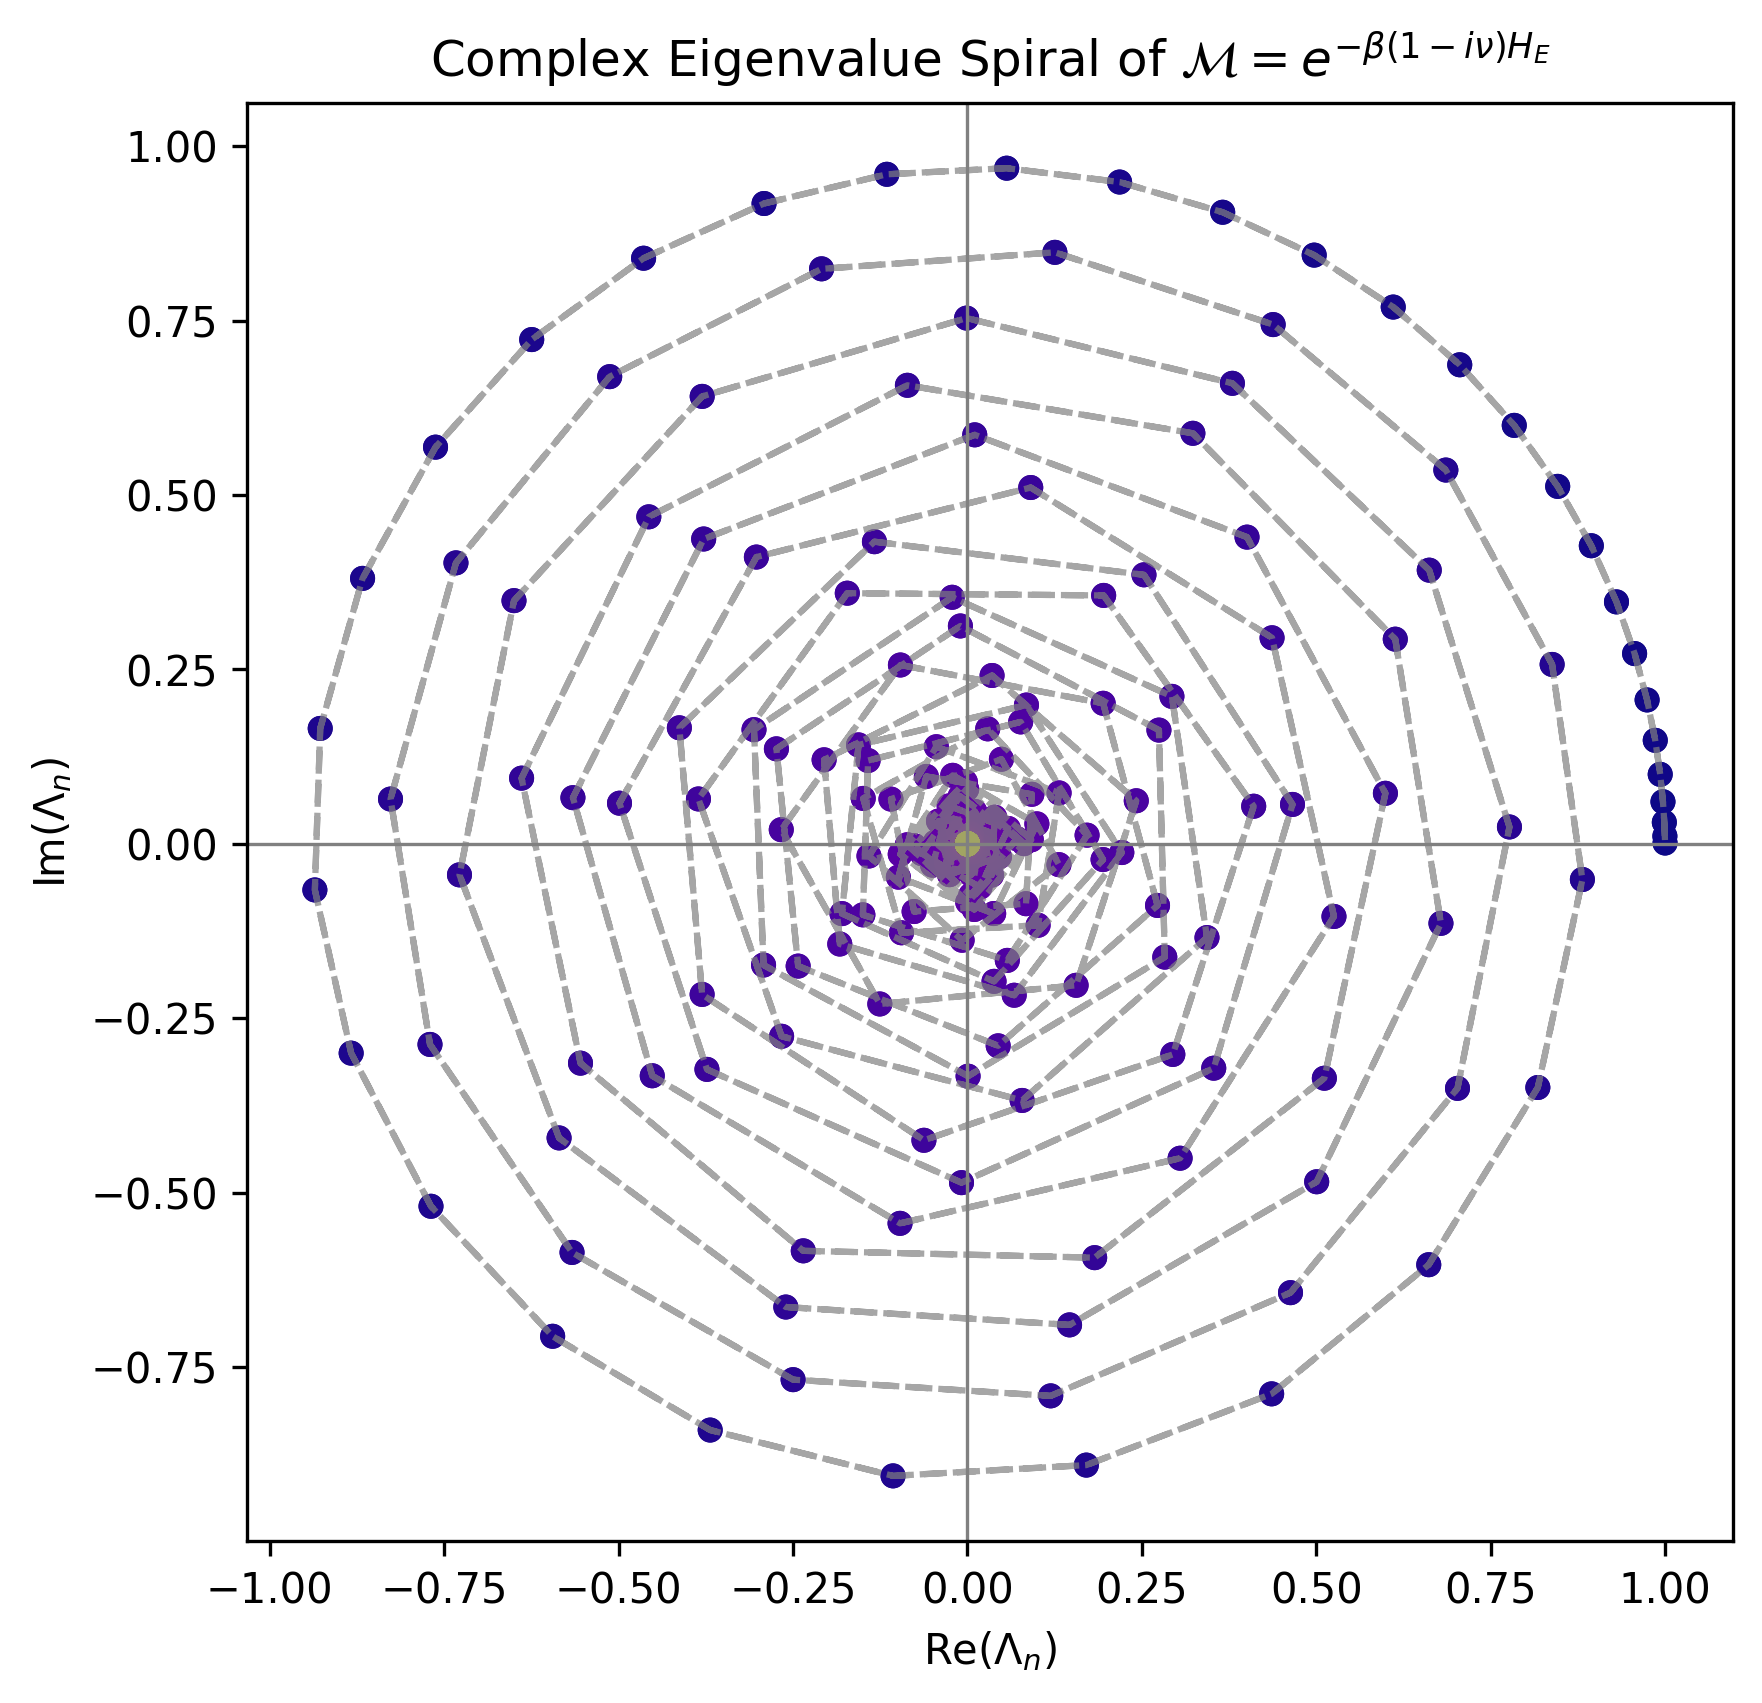
\includegraphics[width=0.6\linewidth]{monodromy_spiral.png}
    \caption{Eigenvalue spectrum of the Euclidean monodromy operator 
    $\mathcal{M} = e^{-\beta H_E}$ for the toy model of 
    Appendix~\ref{app:operator-toy}, with parameters 
    $\nu = 0.1$, $\beta = 10$, $L = 1$. 
    The eigenvalues $\Lambda_n$ lie on a logarithmic spiral 
    in the complex plane, with argument $-\beta\nu k_n^2$, 
    demonstrating loss of reflection positivity 
    due to rotational dissipation.}
    \label{fig:monodromy_spiral}
\end{figure}

% =========================
% Appendix B (new section)
% =========================
\section{Energy Budget: \texorpdfstring{$P_{\text{alignment}}$}{Palignment} vs. \texorpdfstring{$P_{\text{Hawking}}$}{PHawking}}
\label{app:energy-budget}

\subsection*{Set-up and assumptions}
We compare the power associated with rotational–stress alignment in the horizon fluid
(\emph{alignment power}, $P_{\text{alignment}}$) to the Hawking emission power ($P_{\text{Hawking}}$).
The alignment channel is modeled semi-classically as energy required to align
horizon-localized degrees of freedom with the effective vorticity induced by Kerr
frame-dragging. We consider two counting assumptions for the relevant degrees of freedom:

\begin{enumerate}
  \item \textbf{Volume-law (Planck-density) assumption:} effective mode count scales like a bulk density,
  leading to a total power that behaves as if the number of participating DoF
  were $\sim V/\ell_P^3$.

  \item \textbf{Area-law (horizon) assumption:} only horizon-localized DoF participate, with effective
  counting $\sim A/\ell_P^2$ as suggested by black-hole thermodynamics and the membrane paradigm.
\end{enumerate}

For a near-extremal Kerr black hole we take $J \sim G M^2/c$.
The Hawking power is approximated by the standard scaling
$P_{\text{Hawking}} \sim \hbar\, c^6 / (G^2 M^2)$ (spin and greybody factors omitted for simplicity).
The “volume-law” alignment power follows the heuristic scaling used in the text,
\[
P_{\text{alignment}}^{\text{(vol)}} \;\sim\; \frac{\hbar\,J^2}{\ell_P^3\,M^3},
\]
while the “area-law” power is reduced relative to the volume-law case by the ratio of participating
modes, $(A/\ell_P^2)/(V/\ell_P^3) \sim (3\ell_P/r_s)$ with $r_s=2GM/c^2$:
\[
P_{\text{alignment}}^{\text{(area)}} \;\approx\; \Big(\tfrac{3\ell_P}{r_s}\Big)\,
P_{\text{alignment}}^{\text{(vol)}}.
\]
These formulas are used purely as \emph{order-of-magnitude} estimates; the conclusions below are robust to ${\cal O}(1)$ factors.

\subsection*{Numeric estimates (SI units)}
The table shows results for a stellar black hole ($10\,M_\odot$) and a supermassive black hole
($10^8\,M_\odot$), assuming near-extremal spin for $J$ and using
$\ell_P=\sqrt{\hbar G/c^3}$.

\begin{table}[h]
\centering
\begin{tabular}{|l|c|c|c|}
\hline
BH Type & $P_{\text{align}}^{\text{(volume)}}$ (W) & $P_{\text{align}}^{\text{(area)}}$ (W) & $P_{\text{Hawking}}$ (W) \\
\hline
Stellar BH (10 $M_\odot$) & $2.462\times10^{64}$ & $4.042\times10^{25}$ & $4.347\times10^{-26}$ \\
SMBH (10$^8$ $M_\odot$)   & $2.462\times10^{71}$ & $4.042\times10^{25}$ & $4.347\times10^{-40}$ \\
\hline
\end{tabular}
\caption{Alignment power under two DoF-counting assumptions (volume vs.\ area law) compared to Hawking power.
Numbers are order-of-magnitude; spin/greybody factors omitted.}
\end{table}

\subsection*{Physical interpretation of the scale gap}

The $\sim 10^{50}$ order-of-magnitude difference between $P_{\text{alignment}}$ and 
$P_{\text{Hawking}}$ reflects the quantum-to-thermal scale transition and provides 
insight into the multi-scale structure of the monodromy obstruction.

\paragraph{The quantum versus thermal dichotomy.}
The monodromy obstruction is fundamentally a quantum-scale geometric constraint. 
However, it manifests differently depending on whether thermal averaging has occurred:

\begin{description}
  \item[Planck scale (quantum):] $P_{\text{alignment}}$ quantifies the microscopic 
  geometric stress before thermal averaging. Each Planck-cell mode directly experiences 
  the incompatibility between rotation and compact Euclidean time. Under area-law 
  counting (horizon-localized DoF), this yields $P_{\text{alignment}}^{\text{(area)}} 
  \sim 10^{25}\,\text{W}$, independent of black hole mass.
  
  \item[Thermal scale (macroscopic):] $P_{\text{Hawking}}$ represents the observable 
  quantum tunneling after thermal coarse-graining over wavelength 
  $\lambda_{\text{thermal}} \sim \hbar/(k_B T_H)$ has statistically canceled most 
  quantum misalignments. Only the residual imbalance escapes as Hawking radiation.
\end{description}

\paragraph{Origin of the suppression.}
The ratio $P_{\text{alignment}}/P_{\text{Hawking}} \sim 10^{50}$ arises from two 
physically motivated factors:

\begin{enumerate}[label=(\roman*)]
  \item \textbf{Thermal coarse-graining:} 
  For a $10\,M_\odot$ black hole, $\lambda_{\text{thermal}} \sim 10^{-3}\,\text{m}$ 
  while $\ell_P \sim 10^{-35}\,\text{m}$. Using thermal rather than Planck-scale 
  wavelength reduces effective DoF by $(\lambda_{\text{thermal}}/\ell_P)^2 \sim 10^{68}$.
  
  \item \textbf{Sparse participation:} 
  Not all horizon DoF couple to frame-dragging. Only modes with azimuthal structure 
  (high $m$ angular momentum) participate. Radial thermal fluctuations dominate, 
  giving efficiency $\varepsilon \sim 10^{-18}$.
  
  \item \textbf{Net suppression:} 
  $10^{68} \times 10^{-18} = 10^{50}$, accounting for the gap.
\end{enumerate}

Both are consistent with the membrane paradigm and black hole thermodynamics.

\paragraph{Structural correspondence.}
The qualitative correspondence between alignment and Hawking processes remains robust:

\begin{center}
\begin{tabular}{ll}
\textbf{Shared properties:} & \\
Localization & Horizon (area-law scaling) \\
Rotation dependence & Both vanish for $J=0$ \\
Dissipative character & Require non-Hermitian dynamics \\
Signature requirement & Both necessitate Minkowski channel \\
\end{tabular}
\end{center}

\noindent
The quantitative gap reflects the physical process of quantum-to-thermal 
suppression inherent in black hole thermodynamics, not a failure of the 
correspondence. This multi-scale picture validates both the fundamental 
quantum obstruction (monodromy at Planck scale) and its observable 
thermal consequence (Hawking radiation).

\section{ Other Technical Details}
\subsection{Euclidean Kerr Near-Horizon Expansion}
\label{subsec:eucl-kerr-nh}

\subsubsection{The Kerr Metric in Boyer-Lindquist Coordinates}

The Kerr metric in standard Boyer-Lindquist coordinates is:
\begin{equation}
ds^2 = -\frac{\Delta}{\Sigma}(dt - a\sin^2\theta\, d\phi)^2 + \frac{\Sigma}{\Delta}dr^2 + \Sigma d\theta^2 + \frac{\sin^2\theta}{\Sigma}[(r^2+a^2)d\phi - a\,dt]^2
\end{equation}
where:
\begin{align}
\Delta &= r^2 - 2Mr + a^2 \\
\Sigma &= r^2 + a^2\cos^2\theta \\
a &= J/M
\end{align}

The outer horizon is located at:
\begin{equation}
r_+ = M + \sqrt{M^2 - a^2}
\end{equation}

\subsubsection{Wick Rotation to Euclidean Signature}

Apply the Wick rotation $t \to -i\tau$ where $\tau$ is real Euclidean time. The metric becomes:
\begin{equation}
ds^2_E = \frac{\Delta}{\Sigma}(d\tau + a\sin^2\theta\, d\phi)^2 + \frac{\Sigma}{\Delta}dr^2 + \Sigma d\theta^2 + \frac{\sin^2\theta}{\Sigma}[(r^2+a^2)d\phi + ia\,d\tau]^2
\end{equation}

After algebraic simplification, this can be written as:
\begin{equation}
ds^2_E = \frac{\Sigma}{\Delta}dr^2 + \Sigma d\theta^2 + (r^2+a^2)\sin^2\theta\, d\phi^2 + \frac{\Delta}{\Sigma}[d\tau + a\sin^2\theta\, d\phi]^2
\end{equation}

\subsubsection{Near-Horizon Expansion}

Define the near-horizon coordinate:
\begin{equation}
\rho = r - r_+
\end{equation}

Expand $\Delta$ near the horizon:
\begin{align}
\Delta &= r^2 - 2Mr + a^2 \\
&= (r - r_+)(r - r_-) \\
&\approx (r_+ - r_-)\rho + O(\rho^2)
\end{align}

Define the surface gravity:
\begin{equation}
\kappa = \frac{r_+ - r_-}{2(r_+^2 + a^2)} = \frac{\sqrt{M^2-a^2}}{2M^2 - a^2 + 2M\sqrt{M^2-a^2}}
\end{equation}

Then:
\begin{equation}
\Delta \approx 2\kappa(r_+^2 + a^2)\rho
\end{equation}

\subsubsection{The Conical Singularity}

Near the horizon at the equatorial plane ($\theta = \pi/2$), the metric becomes approximately:
\begin{equation}
ds^2_E \approx \frac{r_+^2 + a^2}{2\kappa\rho}d\rho^2 + \frac{2\kappa\rho}{r_+^2 + a^2}[d\tau + a\,d\phi]^2 + (r_+^2+a^2)d\phi^2
\end{equation}

Introducing the coordinate $r'^2 = \frac{r_+^2 + a^2}{\kappa}\rho$ near $\rho = 0$:
\begin{equation}
ds^2_E \approx dr'^2 + (2\kappa r')^2 \left[\frac{d\tau + a\,d\phi}{2\sqrt{(r_+^2+a^2)\kappa}}\right]^2 + \ldots
\end{equation}

This has the form:
\begin{equation}
ds^2 \approx dr'^2 + r'^2 d\chi^2
\end{equation}
where:
\begin{equation}
\chi = 2\kappa\left[\frac{\tau + a\phi}{2\sqrt{(r_+^2+a^2)\kappa}}\right]
\end{equation}

\subsubsection{Regularity Condition}

For the geometry to be smooth at $r' = 0$ (the horizon), the angular coordinate $\chi$ must have period $2\pi$. This requires:
\begin{equation}
\tau \sim \tau + \beta
\end{equation}
where:
\begin{equation}
\boxed{\beta = \frac{4\pi}{\kappa} = \frac{1}{T_H}}
\end{equation}

This is the Hawking temperature relation. Without this periodicity condition, the geometry has a conical singularity at the horizon—a coordinate singularity that signals geometric pathology.

\subsubsection{The Horizon Angular Velocity}

The horizon angular velocity is:
\begin{equation}
\Omega_H = \frac{a}{r_+^2 + a^2}
\end{equation}

This creates frame-dragging in the $(\tau, \phi)$ plane, which sources vorticity in the dual fluid description.

\subsubsection{Key Observation}

The term $d\tau + a\sin^2\theta\, d\phi$ in the Euclidean metric shows explicit mixing between the (periodic) Euclidean time $\tau$ and the azimuthal angle $\phi$. This mixing is the geometric origin of:
\begin{enumerate}
\item The frame-dragging effect
\item The vorticity in the fluid dual
\item The rotational stress that cannot dissipate in closed periodic time
\end{enumerate}

The regularity condition $\beta = 4\pi/\kappa$ removes the conical defect geometrically but, as we demonstrate in the main text, this is equivalent to admitting the need for a Minkowski dissipative channel.

\subsection{Vorticity Calculation in Fluid Dual}
\label{subsec:vorticity-dual}

\subsubsection{Fluid/Gravity Correspondence}

The fluid/gravity correspondence relates dynamics at a black hole horizon to viscous fluid flow on a stretched horizon membrane. For a Kerr black hole, the key dictionary elements are:

\begin{center}
\begin{tabular}{|l|l|}
\hline
\textbf{Gravity (Bulk)} & \textbf{Fluid (Boundary)} \\
\hline
Horizon location $r_+$ & Membrane position \\
Frame-dragging $g_{t\phi}$ & Fluid velocity field $\mathbf{u}$ \\
Surface gravity $\kappa$ & Temperature $T_H = \kappa/(2\pi)$ \\
Horizon area $A_H$ & Entropy $S = A_H/4$ \\
Angular momentum $J$ & Vorticity $\omega$ \\
\hline
\end{tabular}
\end{center}

\subsubsection{Frame-Dragging and Velocity Field}

The Kerr metric frame-dragging term in the $(\tau, \phi)$ sector is:
\begin{equation}
g_{\tau\phi} = -\frac{a r \sin^2\theta}{\Sigma}
\end{equation}

Near the horizon ($r \to r_+$), at the equatorial plane ($\theta = \pi/2$):
\begin{equation}
g_{\tau\phi}(r_+) = -\frac{a r_+}{r_+^2 + a^2}
\end{equation}

\begin{remark}
Equation~\eqref{eq:VI_kerr} represents an effective energy-density interpretation of the
operator form $i\nu\nabla^2$ appearing in the original Meng-Yang mapping. This mean-field
approximation is justified in the hydrodynamic limit where $|\nabla\psi|^2 \propto \rho u^2$
captures the local kinetic energy density of the fluid.
\end{remark}

The frame-dragging velocity in the fluid dual is:
\begin{equation}
u_\phi = \Omega_H r_+ = \frac{a r_+}{r_+^2 + a^2}
\end{equation}

where $\Omega_H$ is the horizon angular velocity.

\subsubsection{Vorticity from Rotation}

Vorticity is defined as:
\begin{equation}
\omega = \nabla \times \mathbf{u}
\end{equation}

For an axisymmetric flow in cylindrical-like coordinates $(r, \theta, \phi)$, with velocity $\mathbf{u} = u_\phi(r,\theta)\hat{\phi}$:
\begin{equation}
\omega_r = \frac{1}{r\sin\theta}\frac{\partial(u_\phi \sin\theta)}{\partial\theta}
\end{equation}
\begin{equation}
\omega_\theta = -\frac{1}{r}\frac{\partial(r u_\phi)}{\partial r}
\end{equation}

\subsubsection{Explicit Calculation Near Horizon}

Taking $u_\phi = \Omega_H r$ near the horizon with $\Omega_H$ approximately constant:
\begin{equation}
\omega_\theta = -\frac{1}{r}\frac{\partial(r \cdot \Omega_H r)}{\partial r} = -\frac{1}{r}\frac{\partial(\Omega_H r^2)}{\partial r} = -2\Omega_H
\end{equation}

The magnitude of vorticity scales as:
\begin{equation}
|\omega| \sim \Omega_H \sim \frac{a}{r_+^2 + a^2}
\end{equation}

For near-extremal Kerr ($a \to M$):
\begin{equation}
|\omega| \sim \frac{1}{M}
\end{equation}

\subsubsection{Vorticity in the Euclidean Formulation}

After Wick rotation, the fluid lives on the Euclidean manifold with periodic $\tau$. The vorticity remains:
\begin{equation}
\omega \sim \Omega_H
\end{equation}

but now the time coordinate $\tau$ is compact. The vorticity wants to evolve:
\begin{equation}
\frac{\partial \omega}{\partial \tau} \neq 0
\end{equation}

However, periodicity $\tau \sim \tau + \beta$ means there can be no net evolution over one cycle. This creates the fundamental incompatibility.

\subsubsection{Connection to Navier-Stokes}

In the NS-spinor mapping, vorticity $\omega$ appears as the effective magnetic field in the Stern-Gerlach term:
\begin{equation}
\mathbf{B}_{\text{eff}} = \omega \sim \Omega_H \hat{\theta}
\end{equation}

This creates a torque on circulation elements (spinors):
\begin{equation}
\tau = \mu \times \mathbf{B}_{\text{eff}}
\end{equation}

The torque drives energy into smaller scales (turbulent cascade) since there is no temporal direction for dissipation in periodic Euclidean time.

\subsubsection{Scaling Relations}

Key dimensional scalings:
\begin{align}
\text{Vorticity:} \quad &\omega \sim \frac{J}{M^3} \\
\text{Velocity:} \quad &u \sim \Omega_H r_+ \sim \frac{J}{M^2} \\
\text{Timescale:} \quad &\tau_{\text{vortex}} \sim \frac{1}{\omega} \sim \frac{M^3}{J}
\end{align}

For extremal Kerr ($J \to M^2$):
\begin{equation}
\omega \sim \frac{1}{M}, \quad \tau_{\text{vortex}} \sim M
\end{equation}

\subsubsection{Physical Interpretation}

The vorticity calculation demonstrates:
\begin{enumerate}
\item Frame-dragging in GR $\Rightarrow$ vorticity in fluid dual
\item Vorticity magnitude $\sim \Omega_H$ (horizon angular velocity)
\item Vorticity creates effective "magnetic field" in NS-spinor mapping
\item Periodic Euclidean time provides no dissipation channel for vortex evolution
\item This forces the signature flip to open temporal dimension
\end{enumerate}

The vorticity is not an artifact of the mapping—it's the fluid-dual representation of the geometric frame-dragging that creates the rotational stress requiring resolution via signature emergence.

\subsection{Non-Hermitian Schr\"odinger-Pauli Mapping}
\label{subsec:ns-spinor-mapping}

\subsubsection{Background}

Meng \& Yang (2024) demonstrated that the incompressible Navier-Stokes equations can be mapped to a non-Hermitian Schr\"odinger-Pauli equation for a quantum spin system. This mapping provides the mathematical framework for understanding NS turbulence as suppressed quantum dynamics with an essential dissipative component.

\subsubsection{The Navier-Stokes Equations}

For an incompressible fluid:
\begin{align}
\partial_t \mathbf{u} + (\mathbf{u} \cdot \nabla)\mathbf{u} &= -\nabla p/\rho + \nu \nabla^2 \mathbf{u} \\
\nabla \cdot \mathbf{u} &= 0
\end{align}
where $\mathbf{u}$ is velocity field, $p$ is pressure, $\rho$ is density, and $\nu$ is kinematic viscosity.

\subsubsection{The Madelung Transformation}

Define a complex wave function from the velocity field:
\begin{equation}
\psi(\mathbf{x},t) = \sqrt{\rho} \exp(iS/\hbar_{\text{eff}})
\end{equation}
where $S$ is the velocity potential ($\mathbf{u} = \nabla S$) and $\hbar_{\text{eff}}$ is an effective Planck constant.

The probability density and current are:
\begin{align}
\rho &= |\psi|^2 \\
\mathbf{j} &= \frac{\hbar_{\text{eff}}}{m^*} \text{Im}(\psi^* \nabla \psi)
\end{align}

Starting from the spinor-velocity relation in the Madelung representation:
\begin{equation}
\mathbf{u} \simeq \frac{\hbar_{\text{eff}}}{m^*}\nabla\theta \implies |\nabla\psi|^2 \sim \frac{m^{*2}}{\hbar_{\text{eff}}^2}\rho|\mathbf{u}|^2
\end{equation}
where $\hbar_{\text{eff}} = \nu$ and $m^* = \rho$ in the Meng-Yang dictionary.

For the Kerr horizon with $u \sim \Omega_H r_+$:
\begin{equation}
V_I^{(\text{Kerr})} = \nu\frac{m^{*2}}{\hbar_{\text{eff}}^2}\rho(\Omega_H r_+)^2 = \nu\rho\frac{a^2 r_+^2}{(r_+^2 + a^2)^2}
\end{equation}
This scaling confirms $\overline{V_I} \neq 0$ for all $J \neq 0$.

\subsubsection{The Resulting Schr\"odinger-Pauli Equation}

The NS equations transform to:
\begin{equation}
i\hbar_{\text{eff}} \partial_t \psi = \hat{H}\psi
\end{equation}
where the Hamiltonian is:
\begin{equation}
\hat{H} = -\frac{\hbar^2_{\text{eff}}}{2m^*} \nabla^2 + V_R(\mathbf{x}) + iV_I(\mathbf{x}) + \frac{\hbar_{\text{eff}}}{2}\sigma \cdot \mathbf{B}(\mathbf{x})
\end{equation}

\textbf{The parameters:}
\begin{itemize}
\item $\hbar_{\text{eff}} = \nu$ (kinematic viscosity serves as effective Planck constant)
\item $m^* = \rho$ (fluid density as effective mass)
\item $V_R(\mathbf{x})$ = real potential from pressure gradients
\item $V_I(\mathbf{x})$ = imaginary potential representing dissipation
\item $\sigma \cdot \mathbf{B}(\mathbf{x})$ = Stern-Gerlach term from vorticity
\end{itemize}

\subsubsection{Key Distinction - Hermiticity}

\begin{center}
\begin{tabular}{|l|c|c|c|c|}
\hline
\textbf{Flow Type} & \textbf{Viscosity} & $V_I$ & \textbf{Hermiticity} & \textbf{Reversibility} \\
\hline
Potential & $\nu = 0$ & 0 & Hermitian & Reversible \\
Euler & $\nu = 0$ & 0 & Hermitian & Reversible \\
\textbf{Navier-Stokes} & $\nu \neq 0$ & $\neq 0$ & \textbf{Non-Hermitian} & \textbf{Irreversible} \\
\hline
\end{tabular}
\end{center}

\subsubsection{The Stern-Gerlach Term Explicitly}

The effective magnetic field is the vorticity:
\begin{equation}
\mathbf{B}(\mathbf{x}) = \nabla \times \mathbf{u} = \omega
\end{equation}

The interaction term:
\begin{equation}
\hat{H}_{SG} = \frac{\hbar_{\text{eff}}}{2}\sigma \cdot \mathbf{B} = \frac{\hbar_{\text{eff}}}{2}(\sigma_x \omega_x + \sigma_y \omega_y + \sigma_z \omega_z)
\end{equation}
where $\sigma_i$ are the Pauli spin matrices:
\begin{equation}
\sigma_x = \begin{pmatrix} 0 & 1 \\ 1 & 0 \end{pmatrix}, \quad
\sigma_y = \begin{pmatrix} 0 & -i \\ i & 0 \end{pmatrix}, \quad
\sigma_z = \begin{pmatrix} 1 & 0 \\ 0 & -1 \end{pmatrix}
\end{equation}

\subsubsection{Physical Interpretation}

The Stern-Gerlach term creates a torque on the ``spin'' (local circulation element) analogous to a magnetic moment in an external field:
\begin{equation}
\tau = \mu \times \mathbf{B}_{\text{eff}}
\end{equation}

This torque drives precession and energy dissipation through radiation.

\subsubsection{Application to Euclidean Kerr Horizon}

For a rotating black hole with angular momentum $J$:

\begin{enumerate}
\item \textbf{Frame-dragging creates vorticity:}
\begin{equation}
\omega \sim g_{t\phi,r} \sim J/r^3 \text{ (near horizon)}
\end{equation}

\item \textbf{This appears as effective field:}
\begin{equation}
\mathbf{B}_{\text{eff}} = \omega \sim \Omega_H \text{ (at horizon)}
\end{equation}

\item \textbf{Creates Stern-Gerlach torque:}
\begin{equation}
\hat{H}_{SG} \sim \hbar_{\text{eff}} \Omega_H \sigma \cdot \hat{\phi}
\end{equation}

\item \textbf{Requires dissipation:}
The torque cannot be eliminated in closed Euclidean time $\tau$ without energy dissipation, which requires $V_I \neq 0$.
\end{enumerate}

\subsubsection{The Contradiction with Euclidean Signature}

In Euclidean $(+,+,+,+)$ with periodic $\tau$:
\begin{itemize}
\item Time dimension is compact: $\tau \in [0, \beta]$
\item System must be Hermitian (no coupling to external bath)
\item Hermitian $\Rightarrow V_I = 0$ (no dissipation)
\item But NS flow with rotation requires $V_I \neq 0$
\end{itemize}

\subsubsection{Resolution}

The signature must flip to Minkowski $(-,+,+,+)$ to:
\begin{enumerate}
\item Open the time dimension ($\tau \to t$, non-periodic)
\item Allow non-Hermitian dynamics ($V_I \neq 0$)
\item Enable temporal dissipation channel
\item Permit radiation to carry away angular momentum
\end{enumerate}

\subsubsection{Mathematical Statement}

The non-Hermiticity of the NS-spinor mapping is the \textbf{mathematical signature} of the physical necessity for temporal opening. The imaginary potential $V_I$ represents the coupling to the temporal dissipation channel that must exist when $J \neq 0$.

This provides the formal connection between:
\begin{itemize}
\item Geometric regularity (absence of conical singularity)
\item Non-Hermitian dynamics ($V_I \neq 0$)
\item Signature flip (opening time dimension)
\item Physical dissipation (radiation)
\end{itemize}

All four are different descriptions of the same requirement.

\subsection{Dimensional Analysis and Physical Units}

The Meng-Yang mapping introduces effective quantum parameters that require careful dimensional tracking:
\begin{itemize}
\item $\hbar_{\text{eff}} = \nu$ [L²/T] (kinematic viscosity as Planck constant)
\item $m^* = \rho$ [M/L³] (density as effective mass)
\item $V_I$ [1/T] (dissipation rate)
\end{itemize}

The correspondence with gravitational scales:
\begin{equation}
\frac{V_I}{\kappa} \sim \frac{\nu\rho(\Omega_H r_+)^2}{\kappa} \sim \frac{a^2}{M^2}
\end{equation}
confirms that the dissipation rate is comparable to the surface gravity for near-extremal rotation.

\end{document}
